In questa esperimento facoltativo è stato descritto e in seguito analizzato il funzionamento dell'oscillatore a rilassamento. Il circuito è rappresentato in Figura \ref{fig:Circuit_FAC2}. Sono stati utilizzati i seguenti componenti:
\begin{itemize}
    \item Amplificatore operazionale a doppia uscita, codice TL082CP
    \item Resistenze $R_1,R_2,R$ a valori da determinare
    \item Condensatore da $100nF,220nF,1\mu F$ in dotazione
\end{itemize}
\begin{figure}[H]
    \centering
    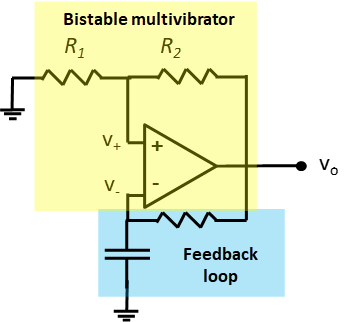
\includegraphics[width=0.6\linewidth]{images/Circuit_fac2.png}
    \caption{Schema circuito}
    \label{fig:Circuit_FAC2}
\end{figure}
Il circuito è alimentato dalla tensione duale: $\pm V_{CC}=\pm10V$
\subsection{Descrizione del funzionamento del circuito}
Un modo semplice per generare onde quadre è forzare un circuito bistabile a cambiare stato periodicamente. Questo può essere ottenuto connettendo un circuito bistabile a una rete di retroazione RC. Questo circuito non ha stati stabili, ed è detto multivibratore astabile.

Si noti che non sono presenti ingressi, ciò comporta che all'accensione dell'alimentazione l'uscita $V_o$ si porta a uno dei due valori di saturazione $L_+$ o $L_-$.
Se per ipotesi l'uscita si trova al valore $L_+$, si ha $V_+=\beta L_+$ (con $\beta = \frac{R1}{R1+R2}$), mentre il condensatore $C$ si carica verso L+ attraverso la resistenza $R$. 
Quando la tensione ai capi del condensatore raggiunge $V_{th}=\beta L_+$, l'uscita $V_o$ commuta verso l'altro stato stabile in cui $V_o = L_-$ e $V_+ =\beta L_-$.
Il condensatore inizia a scaricarsi fino a $V_{tl} = \beta L_-$, dove avviene la successiva commutazione.
Da qui in poi il circuito continua a commutare tra i due stati fino allo spegnimento dell'alimentazione.
\subsection{Dimensionamento del circuito}
Si vuole dimensionare i  componenti $R_1,R_2,R,C$, in modo tale che il circuito risultante abbia frequenza di oscillazione pari a $100Hz$.\\
Il periodo $T$ dell'onda quadra in uscita vale
\begin{equation}
    T=2\tau\ln{\frac{1+\beta}{1-\beta}}
\end{equation}
Dove $\beta=R_1/R_1+R_2$ e $\tau=RC$ costante di tempo. I valori di $R_1,R_2$ sono quelli scelti nel primo esperimento, quindi
\begin{equation*}
    R_1=R_2=10k\Omega\implies\frac{1+\beta}{1-\beta}=3
\end{equation*}
Scelto un valore di capacità tra quelli disponibili, è stato ricavato il valore della resistenza $R$ da
\begin{equation}
    R=\frac{1}{f2C\ln{3}}
\end{equation}
Quindi ponendo $C=100nF$ si è ottenuto
\begin{equation*}
    R = 45511.96\Omega \approx 47k\Omega
\end{equation*}
Riassumiamo nella tabella sotto il dimensionamento del circuito scelto.
\begin{table}[H]
    \centering
    \begin{tabular}{|c|c|}
        \hline
        $R_1$&$10k\Omega$\\\hline
        $R_2$&$10k\Omega$\\\hline
        $R$&$47k\Omega$\\\hline
        $C$&$100nF$\\\hline
    \end{tabular}
\end{table}
\subsection{Risultati}
Sono riportate di seguito le forme d'onda di $v_0,v_{-},v_{+}$, rispettivamente in Figura \ref{fig:FACV0},\ref{fig:FACV-},\ref{fig:FACV+}.
\begin{figure}[H]
    \centering
    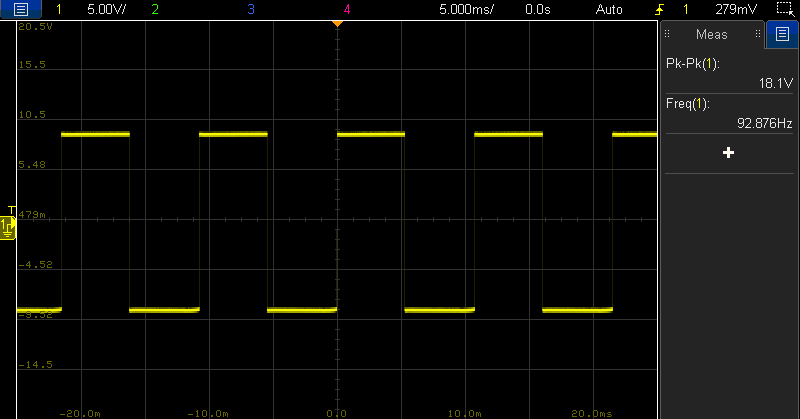
\includegraphics[width=0.7\linewidth]{images/FACV0.png}
    \caption{Forma d'onda presa in $v_0$}
    \label{fig:FACV0}
\end{figure}
\begin{figure}[H]
    \centering
    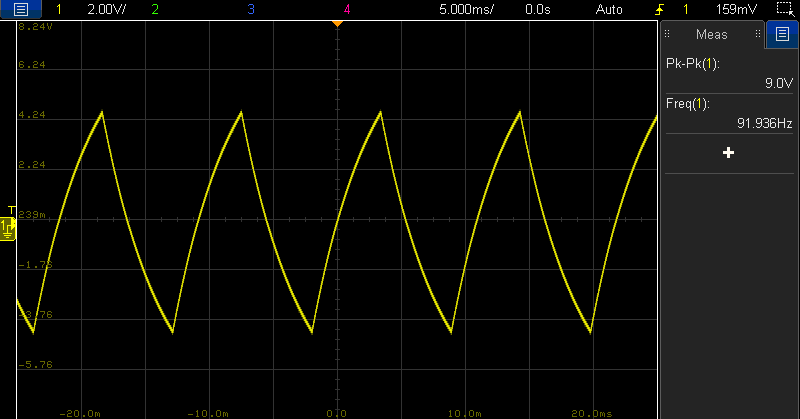
\includegraphics[width=0.7\linewidth]{images/FACV-.png}
    \caption{Forma d'onda presa in $v_-$}
    \label{fig:FACV-}
\end{figure}
\begin{figure}[H]
    \centering
    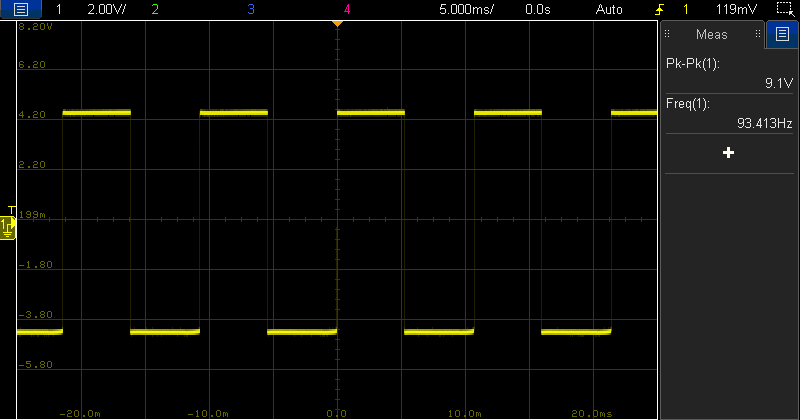
\includegraphics[width=0.7\linewidth]{images/FACV+.png}
    \caption{Forma d'onda presa in $v_+$}
    \label{fig:FACV+}
\end{figure}
\clearpage
\subsection{Elaborazione dati con MATLAB\textregistered\xspace}
Riportiamo in Figura \ref{fig:MatlabPlot} il plotting fatto con MATLAB\textregistered\xspace dei dati campionati con l'oscilloscopio.
\begin{figure}[H]
    \centering
    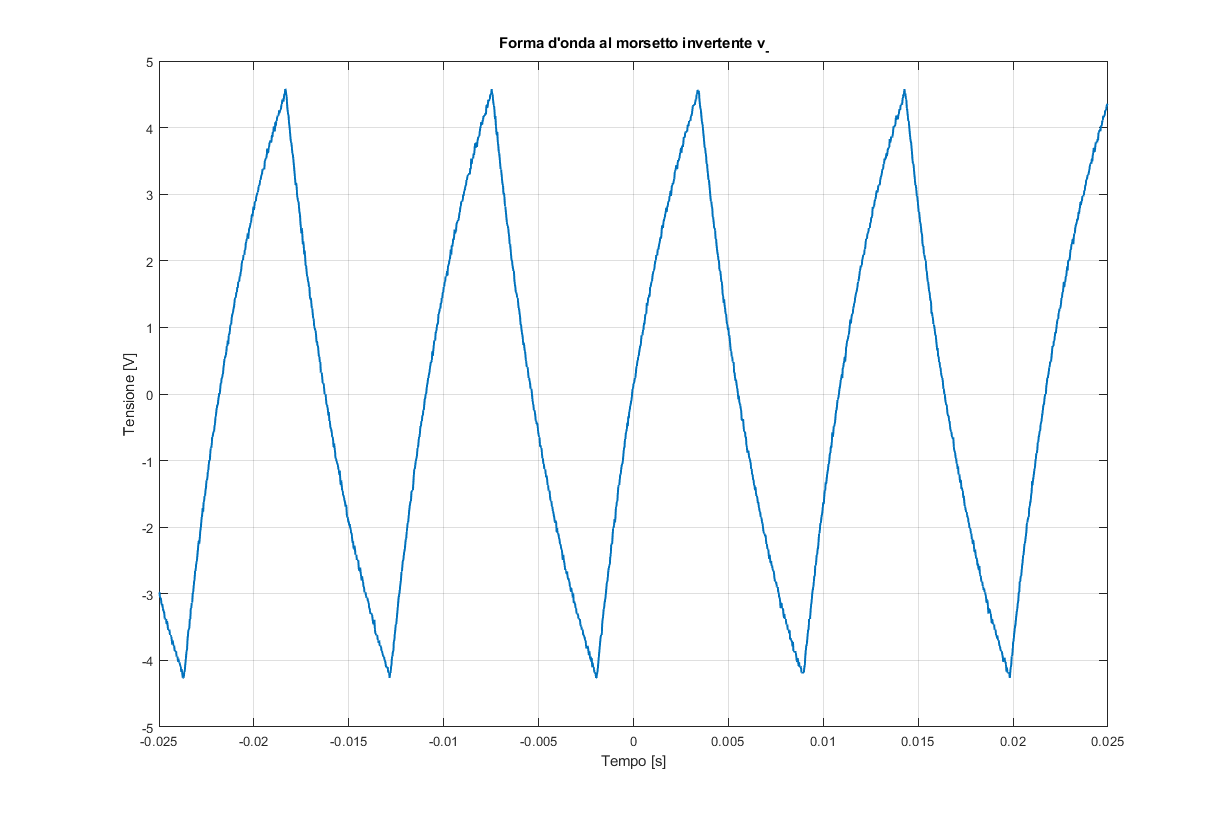
\includegraphics[width=0.6\linewidth]{images/MatlbFac2.png}
    \caption{Plot MATLAB\textregistered\xspace}
    \label{fig:MatlabPlot}
\end{figure}
Il valore di $\tau$ determinato dal dimensionamento del circuito è
\begin{equation*}
    \tau=RC=0.0047 \quad[\Omega F]
\end{equation*}
Tramite la funzione \textit{CurveFitter} di MATLAB\textregistered\xspace abbiamo ricavato un valore alla variabile $\tau$. Il fitting è stato fatto solo su un fronte di salita scelto. Come si vede in Figura \ref{fig:MatlabFit}
\begin{figure}[H]
    \centering
    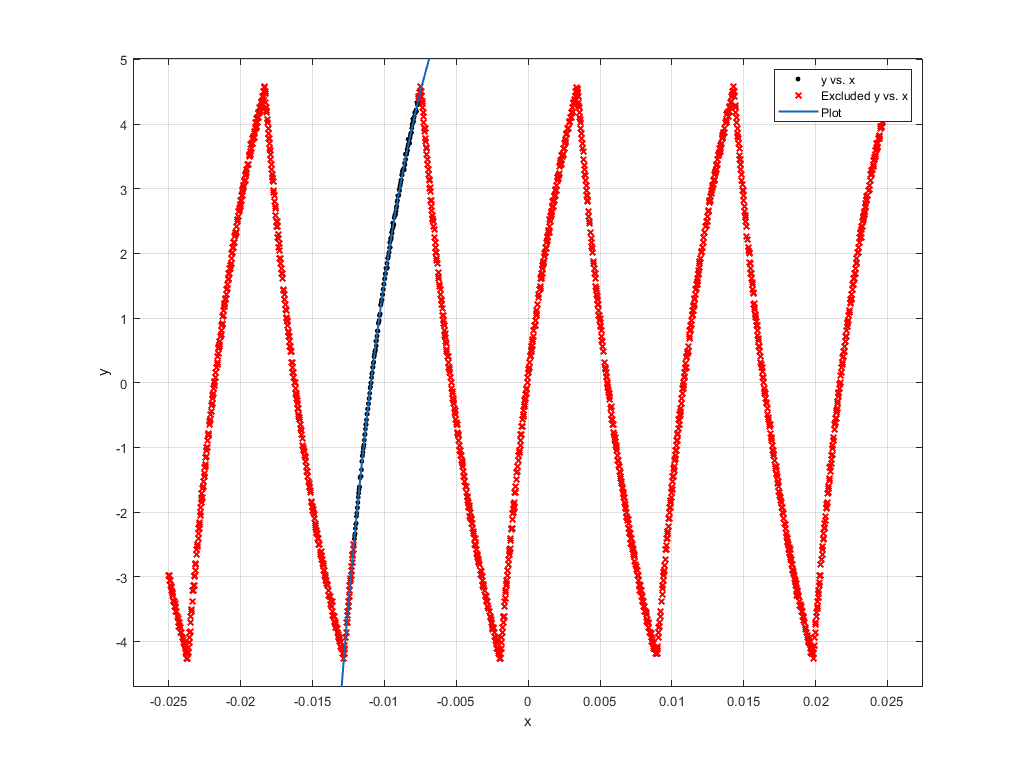
\includegraphics[width=0.6\linewidth]{images/MatlbFIT curve.png}
    \caption{Curve Fitter sui dati campionati}
    \label{fig:MatlabFit}
\end{figure}
Dal fitting abbiamo ricavato il seguente valore di $\tau = 0.004707$.